A system is judged by the quality of the services it offers and its ability to function reliably. Even though reliability of operating systems has been studied for several decades, it remains a major concern today. The characteristics of operating systems which make them unstable are size and complexity. 
\\
Software reliability study shows that 6 to 16 number of errors/1000 executable lines can be found within a module\cite{Basili:1984:SEC:69605.2085, Tanenbaum06canwe}. Linux kernel has over 15 million lines of code. If we assume minimum estimate, Linux kernel has around 90,000 bugs. Researchers have shown that the error rate for device drivers is higher than the error rate for the rest of the kernel\cite{Chou:2001:ESO:502034.502042}. Considering the fact that the operating system predominantly consists of device drivers, the faults in device drivers make the operating system unreliable\cite{Chou:2001:ESO:502034.502042}.

\pagebreak

\section {Problem Statement}

In order to make a system reliable, it is essential that a device driver code does not contain any bug. However, finding all the bugs and fixing them is difficult since bug fixes introduces new lines of code resulting in new bugs. 
\\
In modern operating systems, memory protection is a way to control memory access rights. The memory protection prevents a process from accessing memory that has not been allocated to it. The memory protection prevents a bug within a process from affecting other processes, or the operating system\cite{Denning:1970:VM:356571.356573, Galvin}. Monolithic kernel component do not have the same level of isolation the user level applications have. Unlike user applications, monolithic kernel has hundreds of procedures linked together. As a result, any portion of the kernel can access and potentially overwrite any kernel data structure used by an unrelated component. Such a non-existent isolation between kernel and device driver causes a bug in device drivers to corrupt the memory of the other kernel components. This memory corruption might lead to system crash. Hence the underlying cause of unreliability in the operating system is the tight coupling between device driver and Linux kernel.
\\
In the past, solutions to increase the reliability of a system running monolithic kernel, based on virtualization has been proposed by LeVasseur et. al. \cite{LeVasseur04UnmodifiedDriverReuse}, Tanenbaum et. al.\cite{Tanenbaum06canwe}, Nooks\cite{Swift:2002:NAR:1133373.1133393}, Soltesz et. al. \cite{Soltesz:2007:COS:1272998.1273025}. These solutions improve the reliability of the system by executing device drivers in an isolated environment from the kernel. The use of virtual machines has a well-deserved reputation for extremely good fault isolation. Since none of the virtual machines are aware of the other virtual machines, malfunctioning of one virtual machine cannot spread to the others. Xen hypervisor also provides a similar platform to isolate device driver from the monolithic kernel. The platform is called driver domain \cite{driverdomain}.
\\
Despite the advances in virtualization technology, the overhead of I/O virtualization significantly affects the performance of applications\cite{Barham:2003:XAV:945445.945462, Sugerman:2001:VID:647055.715774, Menon:2006:ONV:1267359.1267361}. In this thesis, we propose and evaluate an optimization for improving the performance of the driver domain under the Xen. 

\pagebreak
  
\section {Proposed Solution} 

In a virtualized environment, all virtual machines run as separate user processes in different address spaces. Thus, to exploit the memory protection capability between virtual machines, xen runs a device driver with a minimalistic kernel in a separate domain, and runs user applications and a kernel in the guest domain. As a result, a device driver is isolated from the Linux kernel, making it impossible for the device driver to corrupt any kernel data structure in the virtual machine running user applications. 

\begin{figure}[!ht]
\centering
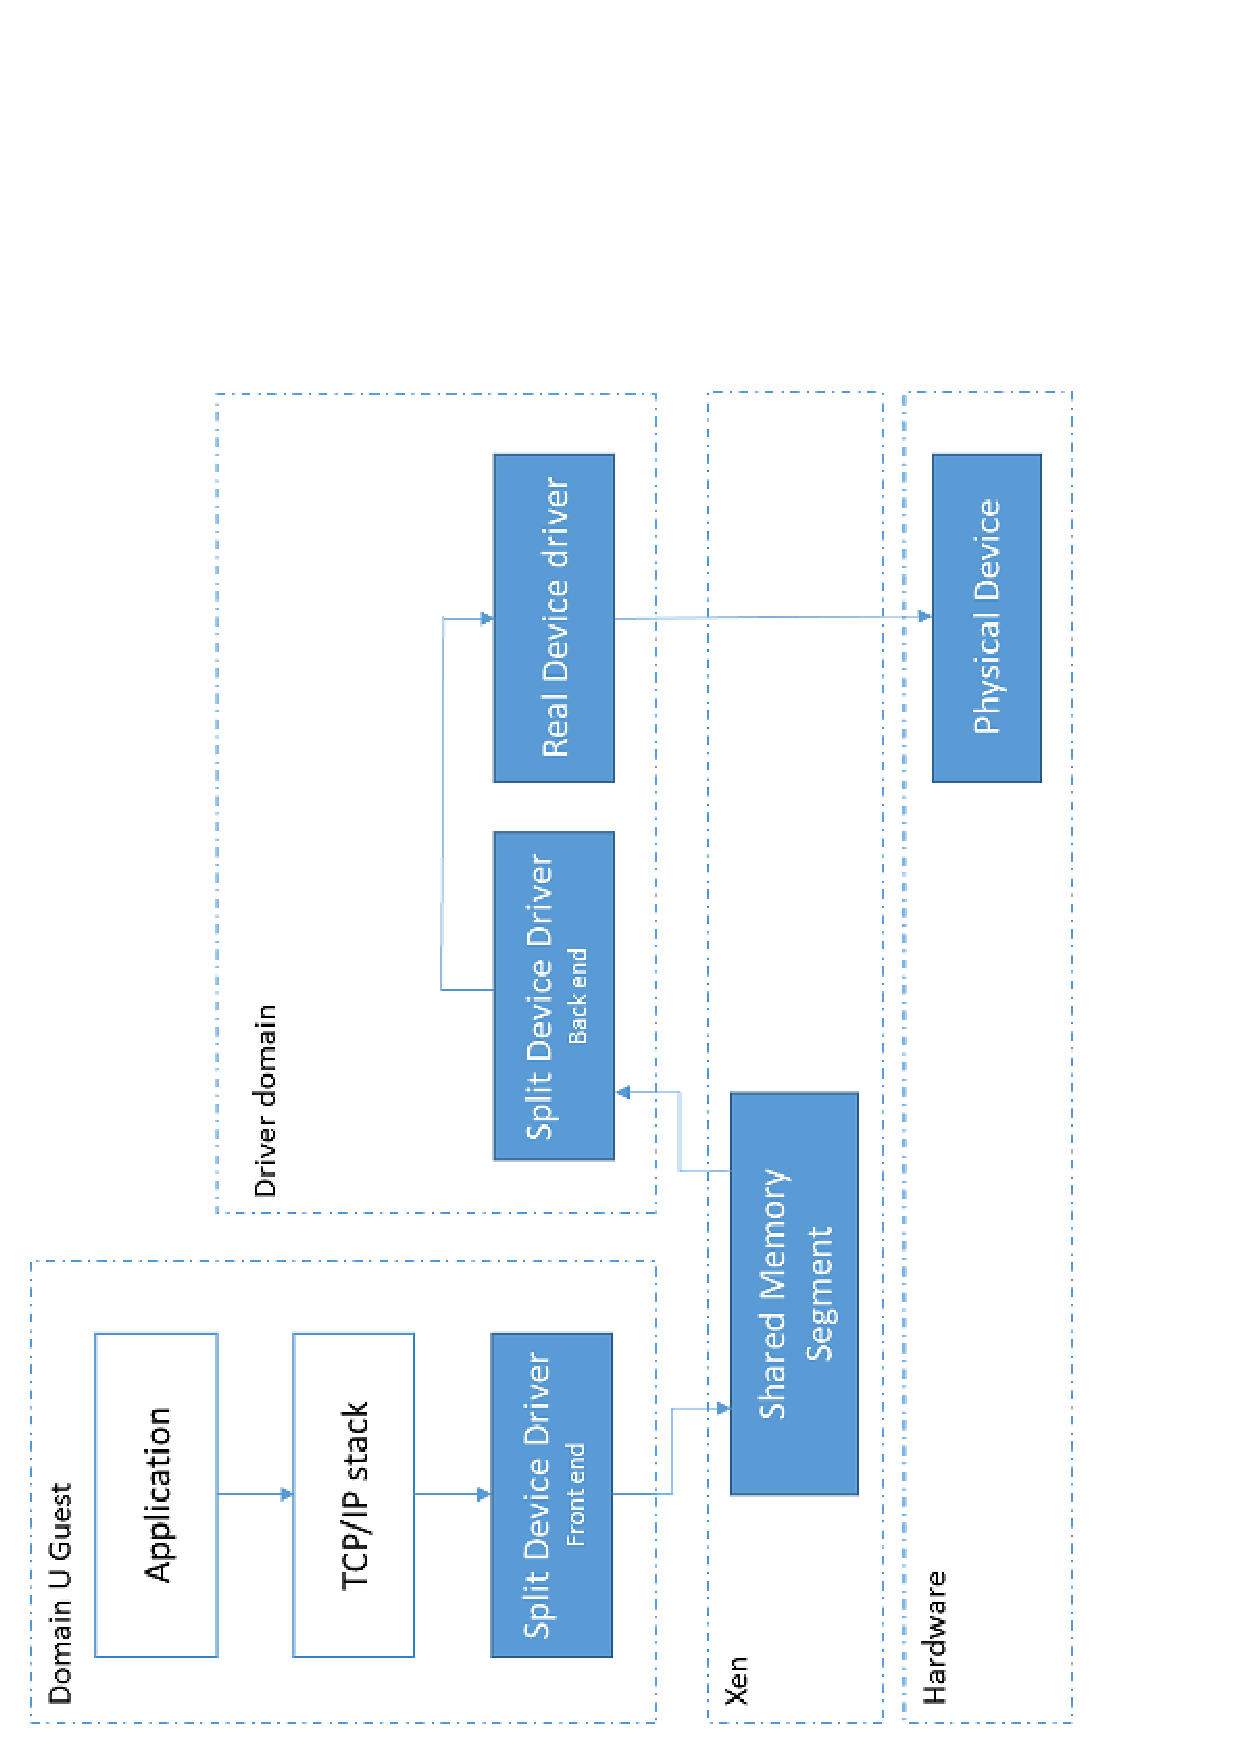
\includegraphics[scale=.35]{xen-split}
\caption{Split device driver model}
\label{fig:xen-split}
\end{figure}

As shown in Figure~\ref{xen-split}, Xen follows a split device driver model. Xen has a front end driver in the guest operating system and a back end driver in the driver domain. The front end and the back end driver transfer data between domains over a channel that is provided by the Xen virtual machine monitor. Within the driver domain, back end driver is used to demultiplex incoming data to the device and to multiplex outgoing data between the device and the guest domain\cite{driverdomain}
\\
The Xen design follows an interrupt based approach in the communication channel\cite{Barham:2003:XAV:945445.945462}. This interrupt based model requires the context switches\cite{Barham:2003:XAV:945445.945462}. In a multitasking system, context switch refers to the switching of the CPU from one process or thread to another. Context switch makes multitasking possible. At the same time, context switch causes unavoidable system overhead\cite{Li:2007:QCC:1281700.1281702, Mogul:1991:ECS:106973.106982}. Hence the overhead is caused by the communication channel in the Xen driver domain. 
\\
We propose and implement an alternate approach for improving the performance of the driver domain. Further, we conduct a comparative analysis and evaluate the performances of both the approaches. 

\pagebreak

\section{Core Contributions}

The core contributions of this project are listed below. 

\begin{enumerate}
\item The implementation of the Xen driver domain concept using alternate design. 
\item The performance comparison of the alternate approach with the xen driver domain.
\end{enumerate}

\pagebreak
\section {Organization}

This section gives the organization and roadmap of the thesis.

\begin{enumerate}
\item Chapter 2 gives the background on memory protection, virtualization, Xen Hypervisor, inter-domain communication, processes and threads. 
\item Chapter 3 gives the introduction to design of the system to isolate device driver. 
\item Chapter 4 discusses the detailed design and implementation to isolate device driver. 
\item Chapter 5 evaluates the performance of Independent device driver with different designs.
\item Chapter 6 reviews the related work in the area of kernel fault tolerance.
\item Chapter 7 concludes the report and lists down the topics where this work can be extended.
\end{enumerate}

% ref
\ifbool{toShowBibliography}{\bibliography{references}}{}